\documentclass[conference]{IEEEtran}
% packages
\usepackage{xspace}
\usepackage{hyperref}
\usepackage{todonotes}
\usepackage{tikz}
\usepackage[utf8]{inputenc}

%  commands
% \newcommand{\todo}[1]{$\langle\!\langle$\marginpar[\raggedleft$\triangleright\triangleright\triangleright$]{$\triangleleft\triangleleft\triangleleft$}\textsf{#1}$\rangle\!\rangle$}
\def\CC{{C\nolinebreak[4]\hspace{-.05em}\raisebox{.4ex}{\tiny\bf ++}}}
\def\ea{\,et\,al.\ }

\begin{document}
	
% paper title
\title{Riss Solver Framework v5.05}

% author names and affiliations
% use a multiple column layout for up to three different
% affiliations
\author{
\IEEEauthorblockN{Lucas Kahlert \and Franziska Krüger \and Norbert Manthey \and Aaron Stephan}
\IEEEauthorblockA{Knowledge Representation and Reasoning Group\\TU Dresden, Germany}
}

\maketitle

\def\coprocessor{\textsc{Coprocessor}\xspace}
\def\glucose{\textsc{Glucose~2.2}\xspace}
\def\minisat{\textsc{Minisat~2.2}\xspace}
\def\riss{\textsc{Riss}\xspace}
\def\priss{\textsc{Priss}\xspace}
\def\pcasso{\textsc{Pcasso}\xspace}

% the abstract is optional
\begin{abstract}
The sequential SAT solver \riss combines the Minisat-style solving engine of \glucose with a state-of-the-art preprocessor \textsc{Coprocessor} and adds many modifications to the search process. 
\riss allows to use inprocessing based on \coprocessor.
Based on this \riss, we create a parallel portfolio solver \priss, which allows clause sharing among the incarnations, as well as sharing information about equivalent literals. 
Finally, the search space partitioning SAT solver \pcasso is built on top of \priss, allowing to solve a formula with a portfolio solver, and additionally solve this formula with iterative partitioning where each partition is solved with the portfolio solver \priss, including clause sharing over partitions. 
\end{abstract}

\section{Introduction}

The CDCL solver \riss was first build on the \textsc{Minisat} search engine~\cite{EenS:2003}, and next incorporated the improvements that have been proposed for \glucose ~\cite{AudemardS:2009,Audemard:2012:RRS:2405292.2405308}. 
Afterwards, more search algorithm extensions have been added, for example \todo[color=green]{add KI paper modofications, bi-asserting clauses, otfss, minisat-hacks with publications or solver descriptions}
\riss is furthermore equipped with the preprocessor \textsc{Coprocessor}~\cite{Manthey:2012}, 
that implements most of the recently published formula simplification techniques, ready to be used as inprocessing as well by taking care of learned clauses. 
The parallel simplification techniques of \coprocessor are disables in the used configurations. 
The aim of the solver is to provide a huge set of options on the one hand, to be able to adopt to new SAT applications, with an efficient implementation on the other hand. 

Similarly, we build the parallel solver \priss and \pcasso, which again are highly configurable. 
In \priss, each incarnation of \riss can be configured, and furthermore the properties of information sharing can be set. 
\priss first runs a global formula simplification step, before all search is started in parallel. 
Each solver incarnation can simplify the formula again, where currently only equivalence preserving techniques are enabled. 

Finally, \pcasso uses \priss as base solver, that solve a formula based on iterative partitioning. 
Furthermore, another additional \priss incarnation is added to solve the given formula. 
Similarly to the other two solvers, \pcasso first simplifies the formula with a \coprocessor incarnation before starting parallel search.

The incremental solver interface is currently only supported by \riss. 
\priss supports a similar interface, and can be used to use a parallel portfolio solver as incremental solver. 

The remainder of the document describes only the changes that have been applied to the tools compared to their previous versions of 2014.

\section{Modifications of Riss and Coprocessor}

\textsc{Riss 5.05} is an extension of \textsc{Riss 4.27}, where a few techniques have been removed to clean the code base, for example \emph{lazy hyper binary resolution}~\cite{precosat}, which has been executed during search. 
On the other hand, many modification have been added, among others ideas that have been proposed in recent \textsc{Minisat}-Hack-Tracks. 
The considered extensions come from the solvers \todo{add added hacks, cirminisat, restartsat, 999ed, minitsat,mipisat}. 
As usual, all novel features are turned off by default, such that the default behavior of the solver does not change too much when modifying the implementation. 
The initialization from \textsc{MinitSAT} has been improved: the activities for decision variables are initialized in geometrically decreasing order. 

Compared to \glucose, the LBD of the currently constructed learnt clause is only re-calculated if a minimization technique modified the clause.
Finally, \riss implements a modified variables on \emph{restricted extended-resolution}~\cite{glucoseER,dedtreff2014}. 
This variant also allows to structually extract binary AND-gates from the formula, to later use this information to reduce learned clauses by replacing both input literals with the output literal of such a gate. 
Finally, another unpublished additional clause minimization technique is added to conflict analysis. 
Removing learnt clauses can be done as in \glucose based on the LBD of the clause, and an dynamic schedule. 
However, the activity based version and the more static schedule of \minisat are also supported, including the ideas of the randomly assigned activity from~\cite{frenchPaper}. 

The implementation of unit propagation has also been improved: 
Instead of storing binary clauses in an extra watch list, as implemented in \glucose, we store all clauses in a common watch list. 
However, each list entry stores a Boolean flag which indicated whether the current clause is binary, such that we just have to work with the \emph{blocking literal}~\cite{minisat21}, and do not need to access the actual clause. 
By using only one watch list, the used memory can be reduced compared to \glucose.

\coprocessor received only little attention. 
Small changes have been applied to the execution order of the simplification techniques, which now all process least occurring literals first (except \emph{bounded variable addition}~\cite{?}). 
Furthermore, \coprocessor now runs all activated simplification techniques twice in the specified order. 

We added an implementation of a elimination routine to remove \emph{resolution asymmetric tautologies} (RAT)~\cite{?}. 
Based on this routine, and the idea of \emph{covered literal elimination}~\cite{MantheyP:KI:2014}, we implemented routines to add a redundant clause, if it subsumes another clause that is present in the formula. 
Hence, \coprocessor allows to perform \emph{vivification}~\cite{?} (or \emph{clause distillation}~\cite{?}) by adding \emph{asymmetric tautologies} that subsume other clauses. 
Similarly, \coprocessor can add \emph{blocked clauses}, \emph{covered clauses}, or \emph{RATs}. 

The implemented extraction of XORs in the formula does not use a detection based on subsumption any longer. 
On the other hand, the XOR reasoning does not only use information about retrieved unit clauses and equivalent literals, but furthermore encodes ternary XORs back into CNF, to allow the resolution based solver to benefit more from this information. 

The generation of DRAT proofs is supported for most implemented simplification techniques and search additions. 

\section{The Parallel Portfolio Solver Priss}

Received clauses can be minimized by \emph{vivification} and reduced clauses can be shared immediately, as proposed in~\cite{siert}. 
Learned clauses are shared after (i) they have been learned, (ii) they have been used in unit propagation~\cite{glucose4-sat2014}, or (iii) after they have been used for conflict analysis again. 
This way, only ``relevant'' learned clauses are shared. 

Before a clause is shared, it has to pass a size filter and an LBD filter. 
These filters can be set to static thresholds. 
However, the thresholds can also be increased dynamically, if not enough clauses are sent. 
Finally, in case not all clauses are selected for sharing (the above (ii) and (iii)), then the filters might not be used, as the clauses turned out to be relevant for the current incarnation already. 

Shared clauses are received by all incarnations, except the sending incarnation. 
Reception is tried before search decisions on search level $0$. 
The activity of received clauses is set to the value of the most recently learnt clause. 
The LBD of the received clause is estimated based on the size to LBD ratio of the current incarnation, as on search level $0$ there are not variable assignments and levels that can be used to determine the actual LBD of the clause. 
Furthermore, received clauses are ignored in the next removal iteration. 
All these options can be specified for each incarnation -- in the submitted version the parameters are fixed as described above. 

For each incarnation in the portfolio, the configuration can be specified on the commandline. 
\todo{continue here! say that most configs use randomization, some inprocessing, some other techniques, biasserting and so on, aim at solving as many different formulas as possible}
\todo{global simplification, can be ignored, then sharing learned clauses is currently disabled (submitted version does not track simplification results to ensure sound sharing with simplification that does not preserve equivalence)}

\section{The Search Space Partitioning Solver Pcasso}

\riss offers all the parameters that are available in \glucose. 
Furthermore, all the techniques that are mentioned above can be enabled or disabled, and the number of execution steps per technique can be limited, as well as variants can be produced. 
The total number of parameters for the solver is 486, where 190 of these parameters are Boolean, and the remaining parameters have either floating point or integer domains. 
% A parameter specification for almost the full parameter set, as well as a smaller specification that can be used to effectively tune the solver is part of the source code of the solver. 
% These specifications can be used for the configuration tools \textsc{SMAC} and \textsc{ParamILS}~\cite{SMAC}.

For the SAT Competition 2014 the formula size limits for the formula simplification techniques have been set, so that these techniques do not consume too much run time.
Next, a set of well performing techniques was determined by a local-search like selection procedure. 
Based with this configuration, the parameters for the search algorithm have been tuned. 
Finally, the search configuration has been combined with the techniques of the formula simplification. 

\section{Incremental SAT Solving with Riss}


\section{Special Algorithms, Data Structures, and Other Features}

\todo{Mention machine leraning frontend}, that can be used over all tools
\begin{itemize}
	\item Reduzierung des Feature-Raums nicht mittels Information Gain Ratio, sondern der Prinicpal Component Analysis --> Vorteil, weniger Dimensionen bei mehr Informationsgehalt, keine Korrelation
	\item klassifikation mittels k-nearest-neighbors, nicht mit einem random-decision-forest
	\item verwendung von k = 1 (nearest-neighbor) --> vermutlich beste wahl (durch testen herausgefunden) bei kleinen, spezialisierten Trainingsdaten (nur application, wenige Familien, 2200 Instanzen), bevorzugung der robustesten configuration --> Cluster enthalten nur einzelne 'andere' Klassen
	\item http://sourceforge.net/projects/libpca/ Libpca (MIT)
	\item http://arma.sourceforge.net/ armaillo (MPL)
\end{itemize}
\section{Implementation details}

\riss and \coprocessor are implemented in \CC. 
All simplification techniques inside \coprocessor are implemented in separate classes to increase the structure of the code. 
\priss and \pcasso implement the parallel code for multi-core architectures with the pthreads library.
 
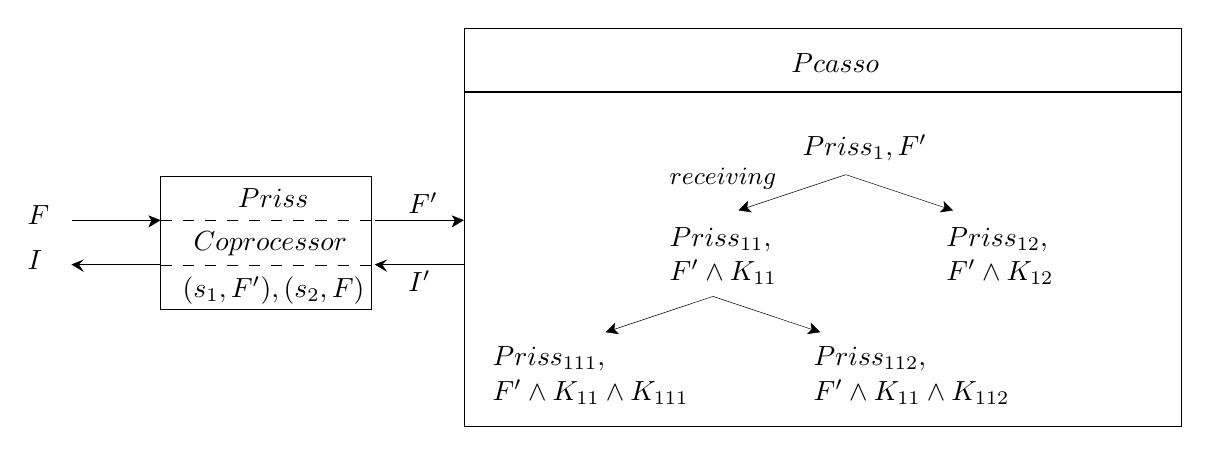
\begin{tikzpicture}[y=0.80pt, x=0.80pt, yscale=-1.000000, xscale=1.000000, inner sep=0pt, outer sep=0pt]

  \path[draw=black,line width=0.160pt,rounded corners=0.0000cm] (370,-453) rectangle (465,-393);
  \path[draw=black,dash pattern=on 4.00pt,line width=0.160pt]   (370,-433)  -- (465,-433);
  \path[draw=black,dash pattern=on 4.00pt,line width=0.160pt]   (370,-413)  -- (465,-413);
  \path[fill=black] (405,-439) node[above right] (text4428) {$Priss$};
  \path[fill=black] (385,-417) node[above right] (text4432) {$Coprocessor$};
  \path[fill=black] (380,-395) node[above right] (text4446) {$(s_1, F'), (s_2, F)$};

  % output arrow
  \begin{scope}[shift={(-130,6.89156)}]
    \path[draw=black,line width=0.160pt] (463,-420) -- (500,-420);
    \path[fill=black] (465,-417) -- (460,-420) -- (465,-422) -- (463,-420) -- cycle;
    \path[draw=black,line width=0.160pt] (465,-417) -- (460,-420) -- (465,-422) -- (463,-420) -- cycle;
  \end{scope}

  % input arrow
  \begin{scope}[shift={(-10,6.89156)}]
    \path[draw=black,line width=0.160pt] (340,-440) -- (376.0260,-440);
    \path[fill=black] (374.7760,-442) -- (379.7760,-440) -- (374.7760,-437) -- (376.0260,-440) -- cycle;
    \path[draw=black,line width=0.160pt] (374.7760,-442) -- (379.7760,-440) -- (374.7760,-437) -- (376.0260,-440) -- cycle;
  \end{scope}

  \path[fill=black] (310,-431) node[above right] (text4466) {$F$};
  \path[fill=black] (310,-411) node[above right] (text4470) {$I$};

  % intermidiate output arrow
  \begin{scope}[shift={(7,6.89156)}]
    \path[draw=black,line width=0.160pt] (463,-420) -- (500,-420);
    \path[fill=black] (465,-417) -- (460,-420) -- (465,-422) -- (463,-420) -- cycle;
    \path[draw=black,line width=0.160pt] (465,-417) -- (460,-420) -- (465,-422) -- (463,-420) -- cycle;
  \end{scope}

  % intermidiate input arrow
  \begin{scope}[shift={(7,6.89156)}]
    \path[draw=black,line width=0.160pt] (460,-440) -- (496.0260,-440);
    \path[fill=black] (494.7760,-442) -- (499.7760,-440) -- (494.7760,-437) -- (496.0260,-440) -- cycle;
    \path[draw=black,line width=0.160pt] (494.7760,-442) -- (499.7760,-440) -- (494.7760,-437) -- (496.0260,-440) -- cycle;
  \end{scope}

  \path[fill=black] (482,-436) node[above right] (text4502) {$F'$};
  \path[fill=black] (482,-401) node[above right] (text4506) {$I'$};

  \path[draw=black,line width=0.160pt,rounded corners=0cm] (507,-520) rectangle (831,-340);

  \path[fill=black] (655,-500) node[above right] (text4498) {$Pcasso$};
  \path[draw=black,line join=miter,line cap=butt,miter limit=4.00,line width=0.435pt] (507,-491) -- (831,-491);

  % level one
  \path[fill=black] (660,-460) node[above right] (text4510) {$Priss_1,  F'$};

  \path[fill=black] (600,-447) node[above right] (text4511) {\small$receiving$};

  % level two
  \begin{scope}[cm={{0.94861,-0.31644,0.31644,0.94861,(255.76474,179.04113)}}]
    \path[draw=black,line width=0.183pt] (555.1339,-466.1446) -- (602.1395,-466.1446);
    \path[shift={(91.12944,-46.14463)},fill=black] (465.2240,-417.5000) -- (460.2240,-420.0000) -- (465.2240,-422.5000) -- (463.9740,-420.0000) -- cycle;
    \path[shift={(91.12944,-46.14463)},draw=black,line width=0.160pt] (465.2240,-417.5000) -- (460.2240,-420.0000) -- (465.2240,-422.5000) -- (463.9740,-420.0000) -- cycle;
  \end{scope}

  \begin{scope}[cm={{-0.94861,-0.31644,-0.31644,0.94861,(1103.2911,179.04114)}}]
    \path[draw=black,line width=0.183pt] (555.1339,-466.1446) -- (602.1395,-466.1446);
    \path[shift={(91.12944,-46.14463)},fill=black] (465.2240,-422.5000) -- (463.9740,-420.0000) -- (465.2240,-417.5000) -- (460.2240,-420.0000) -- cycle;
    \path[shift={(91.12944,-46.14463)},draw=black,line width=0.160pt] (465.2240,-422.5000) -- (463.9740,-420.0000) -- (465.2240,-417.5000) -- (460.2240,-420.0000) -- cycle;
  \end{scope}

  \path[fill=black] (600,-419) node[above right] (text4518) {$Priss_{11},$};
  \path[fill=black] (600,-404) node[above right] (text4519) {$F' \land K_{11}$};
  
  \path[fill=black] (725,-419) node[above right] (text4522) {$Priss_{12},$};
  \path[fill=black] (725,-404) node[above right] (text4523) {$F' \land K_{12}$};


  % level three

  \begin{scope}[shift={(-60,55)},cm={{0.94861,-0.31644,0.31644,0.94861,(255.76474,179.04113)}}]
    \path[draw=black,line width=0.183pt] (555.1339,-466.1446) -- (602.1395,-466.1446);
    \path[shift={(91.12944,-46.14463)},fill=black] (465.2240,-417.5000) -- (460.2240,-420.0000) -- (465.2240,-422.5000) -- (463.9740,-420.0000) -- cycle;
    \path[shift={(91.12944,-46.14463)},draw=black,line width=0.160pt] (465.2240,-417.5000) -- (460.2240,-420.0000) -- (465.2240,-422.5000) -- (463.9740,-420.0000) -- cycle;
  \end{scope}

  \begin{scope}[shift={(-60,55)},cm={{-0.94861,-0.31644,-0.31644,0.94861,(1103.2911,179.04114)}}]
    \path[draw=black,line width=0.183pt] (555.1339,-466.1446) -- (602.1395,-466.1446);
    \path[shift={(91.12944,-46.14463)},fill=black] (465.2240,-422.5000) -- (463.9740,-420.0000) -- (465.2240,-417.5000) -- (460.2240,-420.0000) -- cycle;
    \path[shift={(91.12944,-46.14463)},draw=black,line width=0.160pt] (465.2240,-422.5000) -- (463.9740,-420.0000) -- (465.2240,-417.5000) -- (460.2240,-420.0000) -- cycle;
  \end{scope}

  \path[fill=black] (520,-365) node[above right] (text4530) {$Priss_{111},$};
  \path[fill=black] (520,-350) node[above right] (text4531) {$F' \land K_{11} \land K_{111}$};
  \path[fill=black] (665,-365) node[above right] (text4534) {$Priss_{112},$};
  \path[fill=black] (665,-350) node[above right] (text4535) {$F' \land K_{11} \land K_{112}$};

\end{tikzpicture}

 
\section{SAT Race 2015 Specifics}

All solvers are submitted as a 64-bit binaries. 
The compilation uses the flag ``-O3''. 

The submitted default configuration of \textsc{Riss 5.05} uses the following techniques:
%
BVE, 
FM, 
five iterations of UNHIDE,
CLE,
EE with structural hashing of AND-gates,
XOR reasoning, 
and variable renaming to compact the representation of the formula during search. 
Furthermore, the unpublished learned clause minimization is used, and the activities for decision variables is initialized as described above. 
Finally, during clause removal we keep $1$ percent of the heuristically ``worst'' learned clauses.

In \pcasso, we use different configurations depending on the number of available computational resources. 
In the global \priss incarnation, the first configuration uses the above configuration of \riss, and does not receive any shared information, such that this incarnation behaves exactly as the sequential solver. 
The other configurations of \priss share information,

\todo{sections below are fixed already}

\section{Availability}

All tools in the solver collection are available for research. 
Besides the abovementioned tools, we furthermore provide a perliminary parallel DRAT proof verifier, as well as the model checker \textsc{ShiftBMC} in this package.
The framework can be downloaded from \url{http://tools.computational-logic.org}.

\section*{Acknowledgment}
The author would like to thank the developers of \glucose and \minisat. 
The computational resources to develop, evaluate and configure the SAT solver have been provided by the BWGrid \cite{bwgrid} project and the ZIH of TU Dresden. 
This project is supported by the DFG grant HO 1294/11-1. 



% \bigskip
% What should not be in the system description:
% \begin{enumerate}
%   \item Basic definitions related to SAT. (However, any formal notations used in the description should be defined.)
%   \item Empirical results on the solver's performance.
% \end{enumerate}
% 
\bibliographystyle{IEEEtran}
\bibliography{local}

\end{document}



% more infos

current pcasso call (test tree communication, no parallel priss, no cross link, no priss in pcasso)

./pcasso -threads=2 -model -work-conflicts=-1 -work-timeout=-1 -split-mode=2 -split-timeout=1024 -presel-fac=0.1 -presel-min=64-presel-max=1024 -fail-lit=2 -nec-assign=2 -num-iterat=3 -con-resolv=1 -bin-const -la-heur=4 -presel-heur=2-clause-learn=2 -dir-prior=3 -child-count=7 -shrk-clause -var-eq=3-split-method=1 -split-depth=0 -dseq -h-acc=3 -h-maxcl=7 -h-cl-wg=5-h-upper=10900 -h-lower=0.1 -shpool-size=15000-shclause-size=2 -stop-children -adp-preselS=7 -sort-split -verbosity=1 -verb=1 -print-tree -g-priss-threads=0 -no-use-priss -no-crosslink -pcasso-com-config=small -g-priss-config=delta -quiet ~/cnf/safe-30-h29-unsat.cnf

current priss call: (especially the independent flag can be combined with other configuration presents to run independent solvers in parallel without communication)

./priss -threads=4 -showUnusedParam -pIncSetup=[3]-independent -addSetup -ppconfig="Riss427:plain_XOR:-cp3_iters=2 -ee -cp3_ee_level=3 -cp3_ee_it -rlevel=2 -bve_early" -psetup=delta
